\documentclass{assignment}
\usepackage{amsmath}
\usepackage{lipsum}
\usepackage{multicol}
\usepackage{fancyhdr}
\usepackage{graphicx}
\usepackage{blindtext}
\usepackage[dvipsnames]{xcolor}
\usepackage{enumitem}
\usepackage{cleveref}
\usepackage{color,soul}
\usepackage{amsfonts}
\def\code#1{\texttt{#1}}
\newtheorem{anm}{Anm}

\fancyhf{}% Clear all headers/footers
% \fancyhead[L]{Numeriska Metoder \\ SF1550}\fancyhead[R]{\textbf{Lucas Frykman, Partner2} \\ lfrykman@kth.se \\ partner2}
\fancyhead[L]{Numeriska Metoder \\ SF1550}\fancyhead[R]{\textbf{Lucas Frykman} \\ lfrykman@kth.se}
\fancyfoot[C]{\thepage}
\setlength{\headheight}{26pt}
\pagestyle{fancy}
\thispagestyle{plain}

\begin{document}
\assignmentTitle
% {Lucas Frykman, Partner2}{0210127650, Partner2}
{Lucas Frykman}{0210127650}
{SF1550}
{Olof Runborg}
{assets/KTH_logga.png}
{Numeriska Metoder, grundkurs}
{Projekt}
\textbf{Bakgrund:} Låt $m$ vara antalet yttre noder och $n-m$ antalet inre noder i ett krets. Vi har totalt n noder i kretset
där $k_{ij}$ är konduktansen mellan node $x_i$ och $x_j$ (En symmterisk koppling vilket innebär att $k_{ij}=k_{ji}$). Där resistansen mellan två noder är $r_{ij}=1/k_{ij}$.
\section*{Del 1: Teori}
Vi vill kunna beskriva strömmen i varje node $x_{i}$ som $I_{i}$ med en ekvations system som beror på spänning och konduktansen i kretsen.
Låt $I_{ij}$ vara strömmen mellan mellan node $x_i$ och $x_j$. Låt $U_{i}$ och $U_{j}$ vara spänning i noderna $x_{i}$ och $x_j$ respketiv.
Vi kan börja från ohms lag som säger:
\begin{align}
    I_{ij} = k_{ij}(U_i-U_j) \label{An2}
    \\ \nonumber \Longleftrightarrow 
    \\ \nonumber \sum_{j\leq n}I_{ij} = I_i = k_{i1}(U_i-U_1) + 
    k_{i2}(U_i-U_2) + \dots \label{An3}
    \\ \nonumber \Longleftrightarrow
    \\ I_i = (k_{i1}+k{i2}+\dots k_{in})U_i - U^\top \cdot 
    \begin{pmatrix}
        k_{i1}
        \\ k_{i2}
        \\ \vdots
        \\ k_{in}
    \end{pmatrix}
\end{align}
\\ Varje värde $I_i$ kan beskrivas med följande produkterna
\begin{align*}
    \\ I_1 = &
    \begin{pmatrix}
        \sum_{j\neq 1 \leq n} k_{1j} && -k_{12} &&  -k_{13} && \dots 
    \end{pmatrix} \cdot U 
    \\ I_2 = &
    \begin{pmatrix}
        -k_{21} && \sum_{j\neq 2 \leq n} k_{2j} &&  -k_{23} && \dots
    \end{pmatrix} \cdot U 
    \nonumber
    \\ I_3 = &
    \begin{pmatrix}
        -k_{31} & -k_{32} & \sum_{j\neq 3 \leq n} k_{3j} & \dots
    \end{pmatrix} \cdot U 
    \\ \vdots
\end{align*}

Det här erhåller ekvations systemet $I = KU$
där varje element $\kappa_{ij}$ (obs: grekisk bokstav "kappa") hos matrisen K kan beskrivas som

\begin{align}
    \left\{\begin{matrix} \label{An1}
        \kappa_{ij} = \sum_{j\neq i \leq n}k_{ij} & \forall i=j
        \\ \kappa_{ij} = -k_{ij} = -k_{ji} & \forall i\neq j
    \end{matrix}\right.
\end{align}
\\ \\
\begin{anm} \label{properties}
    En kirschoff matris $A\in \mathbb{R}^{n \times n}$ ska uppfylla
    \\ (i) $a_{ij}=a_{ji}$
    \\ (ii) $ \sum_{j=1}^n a_{ij} = 0$
    \\  (iii) $ a_{ij}\leq 0 \forall i\neq j$
    \\ $K$ uppfyller (i) genom $k_{ij} = k_{ji}$ och (ii) genom $\sum_{j}^n \kappa_{ij} = \overbrace{(\sum_{j\neq i \leq n}k_{ij})}^{\text{diagonal element}} \underbrace{-k_{i1}-k_{i2}\dots}_{-\sum_{j\neq i \leq n}k_{ij}} = 0$   
    \\ och (iii) genom $0 \leq k_{ij} = 1/r_{ij}$ eftersom samtliga resistanser är positiva
\end{anm}

Låt $U_{yttre}$ , $I_{yttre}$ vara potentialer respektiv strömmar till yttre noderna dvs de första m $\begin{pmatrix} x_1, x_2, \cdots, x_m \end{pmatrix}$ noderna.
och $U_{inre}$, $I_{inre}$ vara likaså till de inre noderna.
Vi vill nu härleda matrisen S till $SU_{yttre} = I_{yttre}$
utifrån ekvationssystemet
% define Kij Iyt and Uyt and label them. 
\begin{align}
    \begin{pmatrix}
        I_{yttre}
        \\ I_{inre} 
    \end{pmatrix}
    = 
    \begin{pmatrix}
        K_{11} && K_{12}
        \\ K_{21} && K_{22}
    \end{pmatrix}
    \begin{pmatrix}
        U_{yttre}
        \\ U_{inre}
    \end{pmatrix}
\end{align}
Där $K := \begin{pmatrix}
    K_{11} && K_{12}
    \\ K_{21} && K_{22}
\end{pmatrix}$
där $K_{ab}$ är uppdelningar av matrisen $K$. Låt $^{ab}\kappa_{ij}$ vara elementen till $K_{ab}$ s.a: 
% \begin{align}
%     ^{11}\kappa_{ij} & = \kappa_{ij} \forall i\leq m, j\leq m \label{K11:element}
%     \\ ^{12}\kappa_{i,(j-m)} & = \kappa_{ij} \forall i \leq m, m+1 \leq j \label{K12:element}
%     \\ ^{21}\kappa_{(i-m)j} & = \kappa_{ij} \forall m+1 \leq i, j\leq m \label{K21:element}
%     \\ ^{22}\kappa_{(i-m), (j-m)} & = \kappa_{ij}\forall m+1 \leq i, m+1 \leq j \label{K22:element}
% \end{align}
\begin{align}
    ^{11}\kappa_{ij} & = \kappa_{ij} \forall i\leq m, j\leq m \label{K11:element}
    \\ ^{12}\kappa_{ij} & = \kappa_{i,(j+m)} \forall i \leq m, j \leq n-m \label{K12:element}
    \\ ^{21}\kappa_{ij} & = \kappa_{(i+m),j} \forall i \leq n-m, j\leq m \label{K21:element}
    \\ ^{22}\kappa_{ij} & = \kappa_{(i+m),(j+m)}\forall i \leq n-m, j\leq n-m \label{K22:element}
\end{align}
\begin{anm}\label{Anm: uppdelningar}
    Vi vet följaktligen att $K_{11}=K_{11}^\top$ från \cref{K11:element} eftersom $^{11}\kappa_{ji}=\kappa_{ji}=\kappa_{ij}$, och på liknande vis att $K_{22}=K_{22}^\top$ från \cref{K22:element} eftersom $\kappa_{(i+m),(j+m)}=\kappa_{(j+m),(i+m)}$ och dessutom vet vi att $K_{12} = K_{21}^\top$ eftersom 
    $^{12}\kappa_{ji} = \kappa_{(i+m),j} = ^{21}\kappa_{ij}$
\end{anm}
För de inre noderna gäller Kirchoffs lag som säger att nettoströmmen från en nod utan strömkälla är noll, dvs $I_{inre}= 0$. 
\begin{align} 
    \Longrightarrow
    \begin{pmatrix}
        I_{yttre}
        \\ 0
    \end{pmatrix}
    = 
    \begin{pmatrix}
        K_{11} && K_{12}
        \\ K_{21} && K_{22}
    \end{pmatrix}
    \begin{pmatrix}
        U_{yttre}
        \\ U_{inre}
    \end{pmatrix}
    \\ \nonumber \Longleftrightarrow
    \\ \nonumber K_{11}U_{yttre} + K_{12}U_{inre} = I_{yttre}
    \\ \nonumber K_{21}U_{yttre} + K_{22}U_{inre} = 0
    \\ \nonumber \Longleftrightarrow
    \\ \nonumber K_{11}U_{yttre} + K_{12}U_{inre} = I_{yttre}
    \\ \nonumber U_{inre} = -K_{22}^{-1}K_{21}U_{yttre}
    \\ \nonumber \Longleftrightarrow
    \\ \nonumber K_{11}U_{yttre} - K_{12}(K_{22}^{-1}K_{21}U_{yttre}) = I_{yttre}
    \\ \underbrace{(K_{11} - K_{12}K_{22}^{-1}K_{21})}_{S:=}U_{yttre} = I_{yttre} \label{An4}
\end{align}
Bevis att S uppfyller $(i)$ från \cref{properties}:
\begin{align}
    S^\top = K_{11}^\top - (K_{12}K_{22}^{-1}K_{21})^\top
    \\ \nonumber \text{(Note that from \cref{Anm: uppdelningar} that $K_{11}=K_{11}^\top$}
    \\ \nonumber \Longrightarrow S^\top = K_{11} -(K_{12}K_{22}^{-1}K_{21})^\top
    \\ \nonumber \text{(Note that $AB^\top = B^\top A^\top $)}
    \\ \nonumber \Longrightarrow S^\top = K_{11} - K_{21}^\top (K_{12}K_{22}^{-1})^\top = K_{11} -K_{21}^\top (K_{22}^{-1})^\top K_{12}^\top
    \\ \nonumber \text{(Note that $(A^{-1})^\top = (A^\top)^{-1} $ och $K_{22} = K_{22}^\top$ från \cref{Anm: uppdelningar})}
    \\ \nonumber \Longrightarrow S^\top = K_{11} -K_{21}^\top (K_{22}^\top)^{-1} K_{12}^\top = K_{11} -K_{21}^\top K_{22}^{-1} K_{12}^\top 
    \\ \nonumber \text{(Note that from \cref{Anm: uppdelningar} that $K_{12}^\top = K_{21}$)}
    \\ \Longrightarrow S^\top = S = K_{11}- (K_{12}K_{22}^{-1}K_{21}) && \square
\end{align}
% Reference K11 and K22 to be kirschoff matrixes by def
% Show that K21 and K12 T are the same
\\ Bevis att S uppfyller $(ii)$ från \cref{properties}:
\begin{align}
    \begin{pmatrix}
        K_{11} && K_{12}
        \\ K_{21} && K_{22} 
    \end{pmatrix}
    \begin{pmatrix}
        1_{yttre}
        \\ 1_{inre}
    \end{pmatrix} = 0
    \\ \nonumber \Longleftrightarrow
    \left\{\begin{matrix}
        K_{11}1_{yttre}+K_{12}1_{inre} = 0
        \\ K_{21}1_{yttre}+K_{22}1_{inre} = 0
    \end{matrix}\right.
    \\ \nonumber \Longleftrightarrow
    \left\{\begin{matrix}
        K_{11}1_{yttre}+K_{12}1_{inre} = 0
        \\ 1_{inre} = -K_{22}^{-1}K_{21}1_{yttre}
    \end{matrix}\right.
    \\ \nonumber \Longleftrightarrow
    K_{11}1_{yttre}+K_{12}(-K_{22}^{-1}K_{21}1_{yttre}) = 0
    \\ \nonumber \Longleftrightarrow
    (K_{11}-K_{12}K_{22}^{-1}K_{21})1_{yttre} = 0
    \\ \Longleftrightarrow
    S\cdot1_{yttre} = 0 && \square
\end{align} 

Bevis att $K_{22}$ är inverterbar: 
\\ 
Vi ska först visa att $K$ är positiv definit med $U^\top KU$.
Vi börjar från \cref{An3} och $I = KU$
\begin{align}
    \nonumber
    KU = 
    \begin{pmatrix}
        \sum_{j \leq n} k_{1j} (U_1-U_j)
        \\ \sum_{j\leq n} k_{2j} (U_2-U_j)
        \\ \sum_{j\leq n} k_{3j} (U_3-U_j)
        \\ \vdots
    \end{pmatrix}
    \\ \nonumber \Longleftrightarrow
    U^\top KU = 
    \begin{pmatrix}
        U_1 & U_2 & U_3 \dots
    \end{pmatrix}
    \begin{pmatrix}
        \sum_{j \leq n} k_{1j} (U_1-U_j)
        \\ \sum_{j\leq n} k_{2j} (U_2-U_j)
        \\ \sum_{j\leq n} k_{3j} (U_3-U_j)
        \\ \vdots
    \end{pmatrix}
    \\ \Longleftrightarrow
    U^\top KU = \sum_{i=1}^n\sum_{j=1}^n k_{ij}(U_i^2-U_jU_i) = \sum_{i\neq j}^n k_{ij} (U_i^2-U_jU_i)
    \\ \nonumber -\text{Note that $\sum_{i\neq j}^n k_{ij} (U_i^2-U_jU_i)= \sum_{i\neq j}^n k_{ji} (U_j^2-U_iU_j)$} 
    \\ \Longleftrightarrow U^\top KU =\frac{1}{2}\sum_{i\neq j}k_{ij}(U_i^2-U_jU_i)+k_{ji}(U_j^2-U_iU_j) =  \frac{1}{2}\sum_{i\neq j}k_{ij}(U_i-U_j)^2 \label{positiv_def}
\end{align}
\\ \cref{positiv_def} är endast noll om $U_1=U_2\dots = U_n$ så vi har visat $K$ är positiv definit. 
Med andra ord vi vet $
\begin{pmatrix}
    K_{11} && K_{12}
    \\ K_{21} && K_{22} 
\end{pmatrix}$ är också positiv definit. Låt $U$ anta vektor värdet $U = \begin{pmatrix}
    0
    \\ U_{inre}
\end{pmatrix}$
Om $0<$\cref{positiv_def} då är 
\begin{align}
    U^\top KU =
    \begin{pmatrix}
        0
        \\ U_{inre}
    \end{pmatrix}^\top
    \begin{pmatrix}
        K_{11} && K_{12}
        \\ K_{21} && K_{22} 
    \end{pmatrix}
    \begin{pmatrix}
        0
        \\ U_{inre}
    \end{pmatrix}>0
    \\ = U^\top KU =
    \begin{pmatrix}
        0
        \\ U_{inre}
    \end{pmatrix}^\top
    \begin{pmatrix}
        K_{12} U_{inre}
        \\ K_{22} U_{inre}
    \end{pmatrix}
    = U_{inre}^\top K_{22}U_{inre}>0 \label{K_22 positiv}
\end{align}
Från \cref{K_22 positiv} kan vi dra slutsatsen att $K_{22}$ är positiv definit och därmed inverterbar $\square$

% Enligt \cref{An1} får vi... 

\newpage
\section*{Del 2: Inledande uppgift}
Med $S$ och $K$ definerad från \cref{An1} och \cref{An4} kan vi implementera de som matlab funktioner.

\lstinputlisting[language=Matlab,label = kirschoff_listing, caption=kirschoff implementation $K(k)$]{assets/K.m} 
$k$ matas in som hela konduktans matris till kirschoff implementationen. 
Specifikationen i vår uppgift är att vi har 6 noder i kretsen med 5 kopplingar. Så vi kan 
beskriva hela $k \in \mathbb{R}^{6 \times 6}$ konduktans matrisen med bara 5 konduktanser: $\mathbf{k}=[k_{15},k_{26},k_{56},k_{35},k_{46}]$
Vi ändrar då \cref{kirschoff_listing} efter specifikationen.
\lstinputlisting[language=Matlab,caption=\code{K.m}]{assets/K2.m} 

och som vår $S(k)$ implementation med $m=4$ yttre noder i \cref{S_func}:
\lstinputlisting[language=Matlab,label=S_func,caption=\code{S.m}]{assets/S.m}
Vi använder funktioner ovan för att beräkna 
$S(\mathbf{k})U_{yttre}=I_{yttre}$ när vi matar in
\\ $\mathbf{k} = 
\begin{pmatrix}
    k_{15} \\ k_{26} \\ k_{56} \\ k_{35} \\ k_{46}
\end{pmatrix}=
\begin{pmatrix}
    9.0 \\ 2.5 \\ 1.0 \\ 0.5 \\ 4.5
\end{pmatrix}\cdot 10^{-3}\Omega^{-1} \Longrightarrow 
S(\mathbf{k}) = 
\begin{pmatrix}
    0.0012 && -0.0003 && -0.0004 && -0.0005
   \\ -0.0003 && 0.0017 && -0.0000 && -0.0014
   \\ -0.0004 && -0.0000 && 0.0005 && -0.0000
   \\ -0.0005 && -0.0014 && -0.0000 && 0.0019
\end{pmatrix}
$
\\ Svaret till vår inledande uppgift där $U_{yttre}=[9,0,0,0]^\top$
\\$
S(\mathbf{k})
\cdot
\underbrace{ 
\begin{pmatrix}
    9
    \\ 0
    \\ 0
    \\ 0
\end{pmatrix}}_{U_{yttre}}
= 
\begin{pmatrix}
    0.0107
   \\-0.0024
   \\-0.0039
   \\-0.0044
\end{pmatrix}
$
\newpage
\section*{Del 3: Lösa $\mathbf{k}$}
Anta att vi vill hitta $\mathbf{k}$ s.a vi uppfyller ekvationerna:
\\ $S(\mathbf{k})\cdot
\begin{pmatrix}
    1 & 0 & 0 & 0
\end{pmatrix}^\top = 
\begin{pmatrix}
    1.10 &-0.18&-0.38&-0.57
\end{pmatrix}^\top$
\\$S(\mathbf{k})\cdot
\begin{pmatrix}
    0&1&0&0
\end{pmatrix}^\top = 
\begin{pmatrix}
    -0.19&1.11&-0.16&-0.8
\end{pmatrix}^\top$,
\\$S(\mathbf{k})\cdot
\begin{pmatrix}
    0&0&1&0
\end{pmatrix}^\top = 
\begin{pmatrix}
    -0.37&-0.15&0.95&-0.42
\end{pmatrix}^\top$,
\\$S(\mathbf{k})\cdot
\begin{pmatrix}
    0&0&0&1
\end{pmatrix}^\top = 
\begin{pmatrix}
    -0.55&-0.77&-0.40&1.75
\end{pmatrix}^\top$
\\ Som kan beskrivas som matris produkten 
\begin{align}
    S(\mathbf{k})\cdot I_{4\times 4} = \label{orig_S_0}
        \begin{pmatrix}
            1.10&-0.19&-0.37&-0.55
            \\ -0.18&1.11&-0.15&-0.77
            \\ -0.38&-0.16&0.95&-0.40
            \\ -0.57&-0.8&-0.42&1.75
        \end{pmatrix}:=S_0
\end{align}

Vi vill alltså lösa $S(\mathbf{k})=S_0$
\\ Det här är ett ekvivalent problem med att minimera funktionen $\left\| S(k)-S_0\right\|^2$
\\ Vi kan göra så genom vektor funktionen $F(\mathbf{k})$ som innehåller varje element hos $\left\| S(k)-S_0\right\|^2$ s.a
\begin{align}
    F(\mathbf{k}) = \begin{pmatrix} \label{F function}
        F_1(\mathbf{k})
        \\ F_2(\mathbf{k})
        \\ F_3(\mathbf{k})
        \\ \vdots
        \\ F_{16}(\mathbf{k})
    \end{pmatrix}
    =
    \begin{pmatrix}
        S_{11}(\mathbf{k})-1.10
        \\ S_{21}(\mathbf{k})-(-0.19)
        \\ S_{31}(\mathbf{k})-(-0.37)
        \\ \vdots
        \\ S_{34}(\mathbf{k})-(-0.42)
        \\ S_{44}(\mathbf{k})-1.75
    \end{pmatrix}
\end{align}
där vi kan minimera $\left\|F(\mathbf{k})\right\|^2$ med \hl{\textbf{Gauss-Newton}}.
\\ Vi gör så genom att implementera en approximation av jacobianen till $F(\mathbf{k})$.
\\$J(\mathbf{k})=
\begin{pmatrix}
    \partial_{k_{15}} F_1(\mathbf{k}) & \partial_{k_{26}} F_1(\mathbf{k}) & \partial_{k_{56}} F_1(\mathbf{k}) & \partial_{k_{35}} F_1(\mathbf{k}) & \partial_{k_{46}} F_1(\mathbf{k})
    \\ \partial_{k_{15}} F_2(\mathbf{k}) & \partial_{k_{26}} F_2(\mathbf{k}) & \partial_{k_{56}} F_2(\mathbf{k}) & \partial_{k_{35}} F_2(\mathbf{k}) & \partial_{k_{46}} F_2(\mathbf{k})
    \\ \partial_{k_{15}} F_3(\mathbf{k}) & \partial_{k_{26}} F_3(\mathbf{k}) & \partial_{k_{56}} F_3(\mathbf{k}) & \partial_{k_{35}} F_3(\mathbf{k}) & \partial_{k_{46}} F_3(\mathbf{k})
    \\ \vdots & \vdots & \vdots & \vdots & \vdots
    \\ \partial_{k_{15}} F_{16}(\mathbf{k}) & \partial_{k_{26}} F_{16}(\mathbf{k}) & \partial_{k_{56}} F_{16}(\mathbf{k}) & \partial_{k_{35}} F_{16}(\mathbf{k}) & \partial_{k_{46}} F_{16}(\mathbf{k})
\end{pmatrix}$
\\
\\ Där vi numeriskt approximerar derivatorna med liten h=1e-10:
\\ 
\\ $\partial_{k_{15}} F_j(\mathbf{k}) \approx \frac{F_j(\mathbf{k}+[h,0,0,0,0]) - F_j(\mathbf{k})}{h}$
\\ $\partial_{k_{26}} F_j(\mathbf{k}) \approx \frac{F_j(\mathbf{k}+[0,h,0,0,0]) - F_j(\mathbf{k})}{h}$
\\ $\partial_{k_{56}} F_j(\mathbf{k}) \approx \frac{F_j(\mathbf{k}+[0,0,h,0,0]) - F_j(\mathbf{k})}{h}$
\\ $\partial_{k_{35}} F_j(\mathbf{k}) \approx \frac{F_j(\mathbf{k}+[0,0,0,h,0]) - F_j(\mathbf{k})}{h}$
\\ $\partial_{k_{46}} F_j(\mathbf{k}) \approx \frac{F_j(\mathbf{k}+[0,0,0,0,h]) - F_j(\mathbf{k})}{h}$
\\ Med det här kan vi implementera jacobianen som en matlab funktion:
\lstinputlisting[language=Matlab,caption=\code{J.m}]{assets/J.m} 
Med $J(\mathbf{k})$ och $F(\mathbf{k})$ kan vi applicera \hl{\textbf{Gauss-Newton}} algoritimen \hl{$\mathbf{x_{k+1} = x_{k}- (J(x_k)^\top J(x_k))^{-1}J(x_k)^\top F(x_k)}$}
Där vi itererar tills felet  $\left\| F(\mathbf{k})\right\|^2$ har tillräckligt konvergerat. Dvs vi tar differensen mellan fel mellan iterationer (line 17 \cref{del_3}) 
och vår avbrottskriteria är när den differensen är tillräckligt nära $0$ som ska vara under toleransen 1e-15. Vi börjar med startgissningen $\mathbf{k} = [1,1,1,1,1]^\top$
\lstinputlisting[language=Matlab,label=del_3,caption=\code{del3.m}: Lösningen för $\mathbf{k}$]{assets/del3.m} 
Resultat till \cref{del_3} erhåller för konduktanserna, resistanserna, felkvadratsumman, och iterationer:
\\ $\mathbf{k}\approx$ \hl{$\cdot[1.602107,1.382071,4.345620,1.225035,4.035113]\cdot 10^{-3}\Omega^{-1}$}
\\ $r=1/ \mathbf{k} \approx$ \hl{$[6.241779,7.235517, 2.301168, 8.163030, 2.478246]\cdot 10^{2}\Omega$}
\\ $\left\|F(\mathbf{k})\right\|^2\approx$ \hl{$2\cdot 10^{-9}$}
\\ Som vi fick med \hl{33} iterationer med tolerans $\tau=$1e-15 
\\ \\ \textbf{Störningsanalys:} Vi använder \hl{\textbf{Gauss-Newton}} implementation i \cref{del_3} som löser $\mathbf{k}$ för att skapa en ny funktion $r(S_0)$ med start matris som input och returnerar 
5 resistanser $r = [r_{15},r_{26},r_{56},r_{35},r_{46}]$. Det är alltså $r=1/\mathbf{k}$ som returneras när vi matar in olika matris värde för $S_0$ s.a $S(\mathbf{k})\approx S_0$
\lstinputlisting[language=Matlab,label=listing_r,caption= \code{r\textunderscore mat.m}]{assets/r_mat.m} 
Vi använder den här funktionenf för experimentell störningsanalys genom att beräkna felgränsen
till $r$ för $S_0$ matrisen från \cref{orig_S_0} som
$E_r \approx |r_1-r|+|r_2-r|\dots +|r_{16}-r|$ där vi har 2 procenthetsfel på varje element på $S_0$ från \cref{orig_S_0} 
\\ $r_{1}=r\begin{pmatrix}
    ^0S_{11}\cdot 1.2&^0S_{21}&\dots&^0S_{44}
\end{pmatrix}$
\\ $r_{2}=r\begin{pmatrix}
    ^0S_{11}&^0S_{21}\cdot 1.2&\dots&^0S_{44}
\end{pmatrix}$
\\ \vdots
\\ $r_{16}=r\begin{pmatrix}
    ^0S_{11}&^0S_{21}&\dots&^0S_{44}\cdot 1.2
\end{pmatrix}$
\\
\\ Vi implmenterar beräkningen för $E_r$ genom att iterera över alla element hos $S_0$
\\ \lstinputlisting[language=Matlab,caption=fel\textunderscore analys.m]{assets/fel_analys.m} 
Som resultat får vi $E_r\approx$ \hl{$[21.9133, 25.3506, 27.0083, 26.9429, 17.9062]$}. Felgränsen är störst hos $r_{56}.$
\newpage
\section*{Del 4: Minimera kostnaden}
Vi kan återanvända $r(S_0)$ (d.v.s \cref{listing_r} \code{r\textunderscore mat}) för att definera $\mathbf{r}(\eta)=r(B_0+\eta B_1)$ (anonym funktion på linje 10 \cref{gyllene}).
Där $B_0$ och $B_1$ är två $4 \times 4$ matriser och $\eta \in [0,1]$  
\\ Vi vill minimera priset 
\begin{align*}
    P_{tot}(\eta)=P(\mathbf{r_{15}}(\eta))+P(\mathbf{r_{26}}(\eta))+P(\mathbf{r_{56}}(\eta))+P(\mathbf{r_{35}}(\eta)+P(\mathbf{r_{46}}(\eta))
\end{align*}
\\ där kostnaden för en resistor på $x$ ohm ges av $P(x)=1+10(\frac{x}{1000})^2$
\\ Om vi plottar $P_{tot}(\eta)$ kommer det se ut så här
\begin{figure}[!h] 
    \caption[short]{Plottan till $P_{tot}(\eta)$}
    \begin{center}
        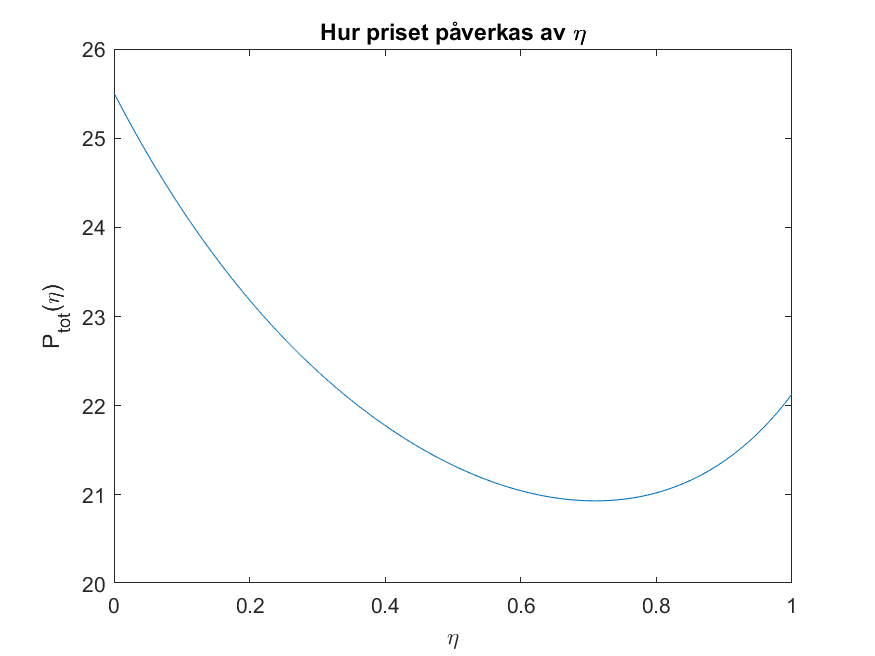
\includegraphics{assets/gyllene_plot.png} \label{plotta}
    \end{center}
\end{figure} 
\\För att minimera total priset $P_{tot}(\eta)$ ska vi använda algoritmen \hl{\textbf{Gyllene Snittet Sökning}} med fel tolerans 1e-10

\lstinputlisting[language=Matlab, label=gyllene, caption=\code{gyllene.m}: Minimera $P_{tot}(\eta)$ med gyllene snittet sökning]{assets/gyllene.m} 
Från \cref{gyllene} får vi lösningen $\eta^*\approx$\hl{$0.72$} i \hl{48} iterationer. Det här stämmer bra med plottan i \cref{plotta}.
\\ För att beräkna felkvadratsumman till $\eta^*$ använder vi $\left\|F(1/\mathbf{r}(\eta^*))\right\|^2$ som vi definerade i \cref{F function} och ersätter matris värdet för $S_0$ med $B_0+\eta^* B_1 $.
Anledningen till att vi matar in $1/\mathbf{r}(\eta^*)$ är till för att få tillbaka $\mathbf{k}$ lösningen som vi hade fått till $S(\mathbf{k})=B_0+\eta^* B_1 $. Så i sista beräkningen får vi:
\\ $P_{tot}(\eta^*) \approx$ \hl{$20.93$}
\\ $\eta^*\approx$\hl{$0.72$}
\\ $\left\|F(1/\mathbf{r}(\eta^*))\right\|^2 \approx$ \hl{$1.34$e-10}

\newpage
\section*{Appendix(kod)}
\lstinputlisting[language=Matlab, caption=\code{F.m}: F(\textbf{k})]{assets/F.m} 
\end{document}